%************************************************
\chapter{Morfologia dei materiali polimerici}\label{ch:Morfologia}
%************************************************
Si vuole riesaminare brevemente i fondamenti della chimica per la realizzazione delle materie polimeriche.
\section{Legami atomici}
I legami chimici possono essere distinti in due categorie:
\begin{description}
\item[Legami forti] sono legami che necessitano di alta energia per potersi sciogliere, sono: legame ionico, legame covalente e legame metallico.
\item[Legami deboli] sono legami di scarsa qualità per cui basta poca energia per sciogliersi, sono: legame idrogeno e \ac{FdW}.
\end{description}
Nello specifico:

\paragraph{Legame ionico} Elementi elettronegativi, tendono a caricarsi più facilmente per completare l'ottetto per divenire stabili. Concetto di verso per la sinistra della tavola periodica: sono propensi a rilasciare elettroni per divenire ioni più stabili.
\begin{itemize}
\item I composti caratterizzati da legame ionico hanno caratteristiche meccaniche decisamente avanzate.
\item I sali sono un tipico esempio di composti a legame ionico.
\end{itemize}

\paragraph{Legame covalente} Nessuno dei due atomi ha sufficiente energia per poter cedere o acquisire un elettrone. Dunque un elettrone viene messo in condivisione al fine di stabilizzare gli elementi.
\begin{itemize}
\item Si formano allora delle molecole. Nei materiali polimerici ci sono molecole di grandi dimensioni dette \textbf{macromolecole}.
\item hanno caratteristiche meccaniche più scarse rispetto al legame ionico.
\end{itemize}

\paragraph{Legame metallico} cationi immersi in una nuvola di elettroni. Con caratteristiche meccaniche decisamente alte.

\subsection{Legame covalente}
La resistenza di un materiale si misura in base a quanta energia devo fornire al fine di spezzare il legame stesso. Infatti, è necessaria parecchia energia per rompere un legame covalente.
Si tratta di un legame direzionale, avviene con una precisa direzione nello spazio.
La direzionalità del legami tende a stare più distanti possibile reciprocamente, questo per via della repulsione elettrostatica. Non è rigido: è un legame forte ma le molecole hanno qualche grado di libertà.
Consentono, ad esempio, la rotazione attorno al legame stesso e qualche piccolo spostamento: flessione, estensione.
La rotazione è permessa solo per legami covalenti singoli; nel caso ci sia legame covalente doppio o triplo no. In quei casi la rotazione è impedita. In realtà se si rompe uno dei due legami, allora la rotazione torna possibile.

I legami doppi non hanno necessità del doppio dell'energia per rompersi: ciò vuol dire che il secondo legame è difficile ma non impossibile.
Si sfrutta tale tecnica per ottenere effettivamente il polimero.

Gli elementi che tipicamente formano legami covalenti (di nostro interesse) sono quelli della tabella \ref{tab:ElementiPolimerici}.

\begin{table}
\centering
\caption{Principali elementi, e quantità di legami covalenti che formano, per lo studio dei materiali polimerici.}
\label{tab:ElementiPolimerici}
\begin{tabularx}{\textwidth}{lX}
\toprule
\textbf{Elemento} & \textbf{Descrizione}\\
\midrule
$C$ & 4 legami covalenti; è l'unico elemento che riesce a creare delle catene di molecole tutte uguali.\\
$Si$ & 4 legami covalenti; o	Non riesce a costituire catene di silicio. Si può costruire una catena di silicio con l'aggiunta di ossigeno, così si formano catene di silicio-ossigeno\\
$H$ & 1 legame covalente\\
$O$ & 2 legami covalenti\\
$N$ & 3 legami covalenti\\
$S$ & 2 legami covalenti. Può anche formare $2 + 2$ legami dativi. Viene impiegato per realizzare elastomeri e altri composti in cui sfruttare questi dativi.\\
$Cl$ & 1 legame covalente; molto elettronegativo.\\
$F$ & 1 legame covalente\\
\bottomrule
\end{tabularx}
\end{table}

Ipotizzando di prendere due qualsiasi elementi $A$, $B$
che formano una molecola \chemfig{A-B}.
Se $A$ è più elettronegativo di $B$, gli elettroni di valenza passeranno più tempo in orbita ad $A$. 
Ciò determina che la molecola presenti una carica localmente negativa per $A$ e positiva per $B$. 
La molecola diventa un dipolo. Resta comunque la direzionalità del legame, in più presenta una carica simile al legame ionico. 
Altro caso di molecola dipolare è l'acqua.
I legami intermolecolari (dovuti al dipolo) permette all'acqua di restare liquida.
Mentre il metano, non avendo questa situazione, ha una temperatura di ebollizione molto bassa.

\subsection{Legami deboli}
Come anticipato in precedenza sono due i principali.
Le \ac{FdW} sono legami molto deboli, di solito intermolecolari. Sono dovute alle interazioni tra nubi elettroniche di una molecola con quelle di un'altra.

Il \textbf{legame idrogeno} assomiglia alle \ac{FdW} ma di più alta qualità. Di solito si forma quando un elemento resta a nucleo scoperto per via del legame covalente, l'elettronegatività locale permette (in particolare all'idrogeno) di legare con altre molecole.
Anche questo è un legame direzionale.

Un esempio di molecole che realizzano legame idrogeno sono le \ac{PA}.

Le \ac{FdW} le si può vedere come una specie di attrito: quando si sottopone le molecole ad una forza di trazione, se ne tira fuori una ma queste forze rendono il compito più difficile. Quindi viene trascinata tutta la matassa di molecole.

Dunque le proprietà meccaniche dipendono:
\begin{itemize}
\item A livello intra-molecolare i legami covalenti sono sollecitati solo dalla rotazione: dunque oppongono poca resistenza.
\item •	A livello inter-molecolare le proprietà sono basse perché i legami tra molecole sono solitamente legami deboli (FdW, legami idrogeno, ibridi ecc\dots)
\end{itemize}

Il motivo che sta dietro alla risposta non rigida ma viscosa, a prove accelerate sta nel fatto che la risposta a tale forza è più veloce di quanto le molecole ruotino tra loro.
Dunque il tempo di applicazione della forza sarà più piccolo di quanto le molecole oscillino, dunque appariranno come ferme alla forza.
Il contrario, se la forza è abbastanza lenta, le oscillazioni delle molecole saranno sufficientemente veloci da potersi adattare alla forza.


\section{Idrocarburi}
Sono molecole composte solamente da $C$ e $H$. 
Ne esistono diverse classi.
\begin{description}
\item[Alcani] sono idrocarburi in cui compaiono solamente legami covalenti singoli nella forma \chemfig{C_nH_{2n+2}}.
\item[Alcheni] sono idrocarburi caratterizzati da un solo doppio legame covalente nella forma \chemfig{C_nH_{2n}}.
\item[Alchimi] sono idrocarburi la quale composizione è del tipo \chemfig{C_nH_{2n-2}}
\item[Dieni] sono idrocarburi caratterizzati da due legami doppi. molto importanti per gli elastomeri.
\end{description}

\subsection{Alcani}
Il carbonio è ibridato $sp3$ per cui la direzione dei legami è ben definita a $109\unit{\degree}$ reciprocamente.
\begin{description}
\item[Metano, $n = 1$] \chemfig{CH_4}
Tutti i legami sono ad una distanza reciproca di $109\unit{\degree}$. La molecola non è planare. Ha punto di ebollizione molto bassa.
\item[Etano, $n=2$] \chemfig{C_2H_6} è gassoso e ha punto di ebollizione più alto del metano per via del maggior peso della molecola.
in più:
\begin{itemize}
\item la rotazione tra i gruppi $CH_3$ (metile) è libera, ma necessita di energia per poter ruotare.
Basta la temperatura ambiente per fornire sufficiente energia per la rotazione.
\item La \textbf{conformazione} con gli idrogeni \textbf{eclissati} (Gli idrogeni sono nascosti) non è incoraggiata.
\item Nella conformazione sfalsata si ha la massima distanza tra gli idrogeni (rotazione di $60\unit{\degree}$).
\end{itemize}
\item[Propano, $n = 3$] \chemfig{C_3H_8} 
Il gruppo \chemfig{CH_2} viene chiamato \textbf{metilene} o \textbf{gruppo metilico}.
\item[Butano, $n = 4$]\chemfig{C_4H_{10}} 
Aumenta il numero degli isomeri, ovvero più configurazioni (non modificabili) della stessa molecola.
Anche in questo caso si possono avere sia conformazioni eclissate che non.
Logicamente l'energia per portare la conformazione eclissata è maggiore di quella sfalsata. La rotazione in questo caso sarà di $180\unit{\degree}$, in mezzo ci saranno altre conformazioni ad energia maggiore (ma non massima). Infatti ci sono delle conformazioni di minimo e massimo relativo
\end{description}

\begin{figure}
\centering
\subfloat[][\emph{Metano}\label{fig:Metano}]%
{%
\begin{minipage}[b]{0.4\textwidth}
\setchemfig{atom sep = 2em}
\chemfig{H-C(-[2]H)(-[6]H)-H}
\end{minipage}%
}\quad
\subfloat[][\emph{Etano}\label{fig:Etano}]%
{%
\begin{minipage}[b]{0.4\textwidth}
\setchemfig{atom sep = 2em}
\chemfig{H-C(-[2]H)(-[6]H)-[@{op,0.75}]C(-[2]H)(-[6]H)-H-[@{cl,0.25}]}
\polymerdelim[delimiters={[]}, indice={\textup{Metile}}]{op}{cl}
\end{minipage}%
}\\
\subfloat[][\emph{Propano}\label{fig:Propano}]%
{%
\begin{minipage}[b]{0.4\textwidth}
\setchemfig{atom sep = 2em}
\chemfig{H-C(-[2]H)(-[6]H)-C(-[2]H)(-[6]H)-C(-[2]H)(-[6]H)-H}
\end{minipage}%
}\quad
\subfloat[][\emph{Butano}\label{fig:Butano}]%
{%
\begin{minipage}[b]{0.4\textwidth}
\setchemfig{atom sep = 2em}
\chemfig{H-C(-[2]H)(-[6]H)-C(-[2]H)(-[6]H)-C(-[2]H)(-[6]H)-C(-[2]H)(-[6]H)-H}
\end{minipage}%
}
\caption{Molecole degli alcani}
\label{fig:Alcani}
\end{figure}

\paragraph{Polietilene}
\begin{figure}
\centering
\setchemfig{atom sep = 2em}
\chemfig{\vphantom{H}-[@{op,0.75}]C(-[2]H)(-[6]H)-C(-[2]H)(-[6]H)-[@{cl,0.25}]}
\polymerdelim[indice=n]{op}{cl}
\caption{Monomero del Polietilene}
\label{fig:PE}
\end{figure}

Alla figura \ref{fig:PE} è un \textbf{Monomero} e il numero in cui questo si ripete nella catena polimerica viene detto \textbf{grado di polimerizzazione}.
In genere nel \ac{PE} il grado di polimerizzazione $n = 10^3 \div 10^5$.

Il polietilene non si trova quasi mai come catena rettilinea, piuttosto si trova come agglomerato detto anche \textbf{conformazione a gomitolo statistico}.
Non è ferma nello spazio: quando riceve energia questa cambia di forma. Il movimento è limitato solamente dalle altre molecole circostanti. (Basta la temperatura ambiente).
Data la conformazione, le proprietà meccaniche sono scarse per via di tale motivo: se ci fosse una catena più o meno rettilinea la resistenza meccanica sarebbe alta.
Invece il gomito, tenderà ad allinearsi, però non offre di sicuro le caratteristiche meccaniche desiderate.

\subsection{Alcheni}
Si presenta con un doppio legame e il carbonio viene ibridato $sp2$ quindi la molecola è planare sta volta.

\begin{description}
\item[Etilene, $n=2$]\chemfig{CH_2=CH_2} 
La sua polimerizzazione da vita al \ac{PE} che si è visto prima.
\item[Propilene, $n=3$] \chemfig{C_3H_6}
Si tratta della molecola del gruppo vinilico
\item[Butilene, $n=4$]\chemfig{C_4H_8}
Il polibutilene non viene impiegato largamente. Piuttosto viene utilizzato il poli-isobuttilene che è un importante elastomero (ad esempio nelle camere d'aria delle bici).
\end{description}

\begin{figure}
\centering
\subfloat[][\emph{Etilene}\label{fig:Etilene}]%
{%
\begin{minipage}[b]{0.4\textwidth}
\setchemfig{atom sep = 2em}
\chemfig{C(-[3]H)(-[5]H)=C(-[1]H)(-[7]H)}
\end{minipage}%
}\quad
\subfloat[][\emph{Propilene}\label{fig:Propilene}]%
{%
\begin{minipage}[b]{0.4\textwidth}
\setchemfig{atom sep = 2em}
\chemfig{C(-[3]H)(-[5]H)=C(-[6]H)-C(-H)(-[1]H)(-[7]H)}
\end{minipage}%
}\\
\subfloat[][\emph{Gruppo Vinilico}\label{fig:Vinile}]%
{%
\begin{minipage}[b]{0.4\textwidth}
\setchemfig{atom sep = 2em}
\chemfig{C(-[3]H)(-[5]H)=C(-[1]H)(-[7]X)}\\
Dove:\\
\begin{tabular}{cl}
$X = H$ & Etilene\\
$X = CH_3$ & Propilene\\
$X = Cl$ & Cloruro di propilene\\
$X = $ altro & Vinile addizionato
\end{tabular}
\end{minipage}%
}
\caption{Alcheni}
\label{fig:Alcheni}
\end{figure}

Tutti i polimeri vinilici costano poco, perché possono essere addizionati molto facilmente dunque c'è letteralmente meno plastica che in altri materiali.


\paragraph{Composti aromatici}
Un esempio di composto aromatico è il \textbf{Benzene}, che sarò una molecola che si ritroverà spesso più avanti.
Risulta molto interessante in quanto è una molecola molto grande, anche in confronto con una catena polimerica ad alto grado di polimerizzazione.
In più essendo i suoi legami \textbf{delocalizzati} per via della risonanza interna, risulta essere una molecola molto rigida.
Infatti, questa non può ruotare per effetto della risonanza. Si dice che abbia legami 1.5.
Una rappresentazione è quella della figura \ref{fig:AnelloBenzenico}.
\begin{figure}
\centering
\setchemfig{atom sep = 2em}
\chemfig{H-C*6(-C(-[5]H)=C(-[7]H)-C(-H)=C(-[1]H)-C(-[3]H)=)} \qquad = \qquad%
\chemfig{**6(------)}
\caption{Anello benzenico}
\label{fig:AnelloBenzenico}
\end{figure}

\subsection{Alchimi}
Il carbonio è ibridato $sp$.
Qui troviamo, di rilevanza per la trattazione della materia, l'\textbf{acetilene} che è un gas che viene utilizzato per le saldature.
Viene polimerizzato in poliacetilene che è un materiale che permette il passaggio di corrente elettrica (come un semiconduttore).

\subsection{Dieni}
Sono idrocarburi identificabili tramite la presenza di due legami doppi.
Importante è il \textbf{Butadiene} che è il materiale più utilizzato per gli elastomeri.

Dalla polimerizzazione si ottiene il \textbf{polibutadiene}.
Si ottiene un polimero con insaturazione al centro.
Infatti questo polimero non conduce.
È un elastomero di sintesi ovvero "\textit{una gomma artificiale}"
La gomma naturale si chiama \textbf{poliisoprene}.
Non siamo in grado di sintetizzare questo tipo di molecola.
Il legame doppio non si può ruotare.


%************************************************
\chapter{Proprietà meccaniche dei polimeri}\label{chp:MeccanicaPolimeri}
%************************************************
Tenendo conto del modello del gomitolo statistico a livello molecolare, vediamo come si classificano le proprietà meccaniche dei polimeri.
\begin{quote}
\emph{Come devono essere "costruiti" i polimeri in modo che si possano ottenere delle proprietà meccaniche interessanti?}
\end{quote}

Un primo modo può essere la strada degli additivi, del resto:\\
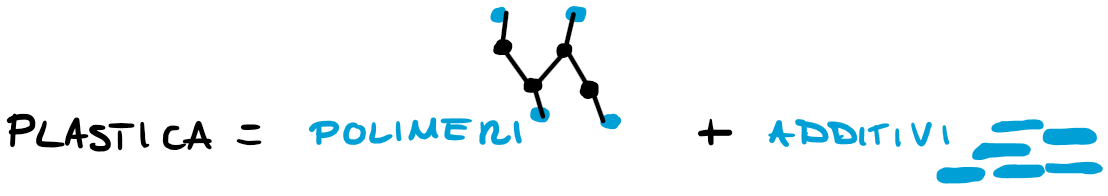
\includegraphics[width = \textwidth]{gfx/Plastica}\\
Un primo additivo usato per irrigidire un struttura polimerica è la fibra di vetro corta.
Vengono infuse nella plastica per migliorare le caratteristiche meccaniche.
Non se ne possono infondere troppe, altrimenti si perde il pregio della formabilità tipica dei materiali plastici.
Le \ac{FVC} vengono aggiunte fino al $40 \div 50\%$ in peso al polimero.

Esistono altre strade per poter migliorare le caratteristiche meccaniche dei polimeri;
\begin{description}
\item[Vincolo geometrico] Vincolare, in qualche modo, il materiale per evitare che il polimero formi la conformazione a gomitolo.
\item[Vincolo chimico] Si può pensare di irrigidire il polimero agendo sulle rotazioni relative delle molecole.
\item[Vincolo di legame] Agire sulla qualità dei legami intermolecolari.
\end{description}

\subsection{Vincolo geometrico}
Per evitare che le molecole ritornino alla forma di gomitolo statistico, si può formare delle fibre di materiale. Così viene limitato ad una certa geometria che, a meno di un piccolo ritorno elastico, non cambia la sua conformazione nel tempo.

Il motivo dell'aumento della resistenza è data dalla forma particolarmente allungata in cui le catene polimeriche vengono forzate.
Infatti, sebbene un minimo resta la conformazione a gomitolo, questo sarà particolarmente allungato. Tale conformazione permetterà alle forze applicate al polimero di agire di più sui legami di buona qualità piuttosto di quelli intermolecolari di qualità più scarsa.
Inoltre la fibra, essendo di piccolo spessore, prevede statisticamente meno difetti lungo la sezione. in pratica si limita la propagazione della frattura.

In particolare, questa pratica viene adottata per il \ac{PE}.

\subsection{Vincolo chimico}
Tenendo a mente la conformazione del \ac{PE}: se in catena principale vengono inseriti degli elementi che costituiscano dei legami covalenti a più alta energia in modo da limitare la rotazione relativa delle molecole.
Ad esempio si possono costituire legami doppi nella catena principale.
Il problema diventa l'instabilità dei legami doppi: tendono ad aprirsi molto facilmente.
Altra soluzione molto sfruttata sta nell'inserire anelli benzenici nella catena principale.
Stiamo parlando del \ac{PET}

\begin{figure}
\centering
\setchemfig{atom sep = 2em}
\chemfig{\vphantom{C}-[@{op,.75}]-C(=[6]O)-(**6(---(-C(=[6]O)-O-CH_2-CH_2-O-[@{cl,.25}])---))}
\polymerdelim[indice = n]{op}{cl}
\caption{Monomero del Polietilene tereftalato}
\label{fig:PET}
\end{figure}

La rigidezza del materiale è donato dall'anello benzenico. Infatti questo racchiude la maggior parte della massa del monomero. Inoltre è particolarmente rigido in quanto non sono permesse le rotazioni delle molecole componenti l'anello per via della risonanza.

Altro esempio di miglioramento del materiale grazie a vincoli chimici è quello del \ac{PPS}.
\begin{figure}
\centering
\setchemfig{atom sep = 2em}
\chemfig{\vphantom{C}-[@{op,.75}]**6(---(-S-[@{cl,.25}])---)}
\polymerdelim[indice = n]{op}{cl}
\caption{Monomero del Polifenilen solfuro}
\label{fig:PPS}
\end{figure}
Le caratteristiche così interessanti sono donate dal fatto che il monomero è praticamente un anello benzenico.
In entrambi i casi si parla di \textbf{Irrigidimento della catena principale}.

Non è l'unica soluzione: si possono aggiungere elementi rinforzanti come sostituenti laterali. In genere si usano elementi pesanti o ingombranti.
In questo caso viene limitato lo scorrimento relativo delle molecole per via dell'ingombro degli anelli benzenici, ad esempio.
Vengono limitate le rotazioni e gli scorrimenti relativi delle molecole per effetto degli ingombri dei sostituenti laterali

\begin{figure}
\centering
\setchemfig{atom sep = 2em}
\chemfig{\vphantom{C}-[@{op,.75}]CH_2-CH(-[6]**6(------))-[@{cl,.25}]}
\polymerdelim[indice = n]{op}{cl}
\caption{Irrigidimento dei sostituenti laterali}
\label{fig:IrrigidimentoLaterali}
\end{figure}

Ma:
\begin{itemize}
\item non si arriva al livello di irrigidimento che si ottiene tramite rinforzo in catena principale.
\item Il materiale ne risulta più fragile (per effetto dei vincoli dati dai sostituenti).
\end{itemize}
Questa tecnica viene detta di \textbf{irrigidimento dei sostituenti laterali}.

\subsection{Vincolo intermolecolare}
Le possibilità in questo caso sono due:
\begin{enumerate}
\item incrementare il numero di legami intermolecolari;
\item incrementare la qualità dei legami intermolecolari;
\end{enumerate}

\paragraph{Incremento numero dei legami}
Prendendo il caso del \ac{PE}: i legami intermolecolari sono di pessima qualità, principalmente \ac{FdW}. Aumentandone il numero risulta in una sommatoria "più lunga" di legami intermolecolari, permettendo un numero di vincoli maggiori.
Vengono realizzate delle catene principali estremamente lunghe.
In questo modo aumentano i "grovigli" che bloccano le catene rispettivamente.
Sempre nel \ac{PE}, si realizzano materiali ad alto grado di polimerizzazione $n \uparrow\uparrow$.
Però aumenta, contemporaneamente, il \ac{PM}:
\begin{equation}
P.M. = P_{\textup{monomero}} * n
\end{equation}

Aumentando il grado di polimerizzazione, le caratteristiche meccaniche aumentano, come si vede in figura \ref{fig:PMMeccanica}.
\begin{quote}
\emph{\dots Però\dots}
\end{quote}

Come si vede dalla figura \ref{fig:ViscPM}, contemporaneamente aumenta anche la viscosità del fluido.

\begin{figure}
\centering
\subfloat[][\emph{Andamento delle caratteristiche meccaniche in funzione del \ac{PM}}\label{fig:PMMeccanica}]
{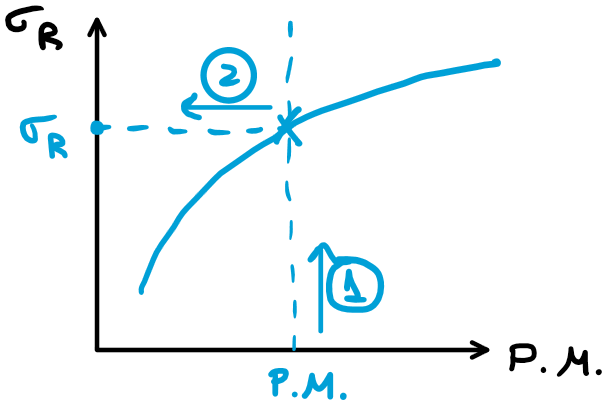
\includegraphics[width = 0.4\textwidth]{gfx/PMMeccanica}}\quad
\subfloat[][\emph{Andamento della viscosità in funzione del \ac{PM}}\label{fig:ViscPM}]
{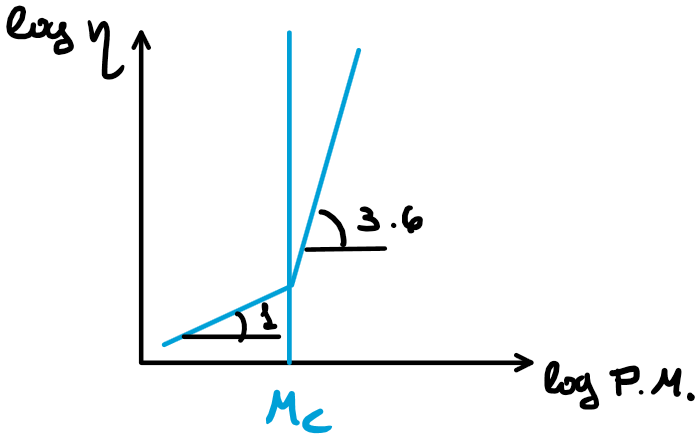
\includegraphics[width = 0.4\textwidth]{gfx/ViscPM}}
\caption{Confronto sull'aumento di \ac{PM} con le caratteristiche meccaniche e viscosità}
\label{fig:ConfPM}
\end{figure}

Nella pratica si fa una scelta in base alla viscosità che serve del polimero, da cui derivano determinate caratteristiche meccaniche.
Ciò è dovuto al fatto che le tecnologie con cui si lavorano i polimeri, necessitano di determinate viscosità per funzionare correttamente.
Ad esempio: nello stampaggio ad iniezione serve una viscosità bassa (per garantire il riempimento dello stampo) altrimenti il fluido non entra.
Mentre per l'estrusione serve una viscosità più alta.

Riassumendo, si sceglie la viscosità sulla base della lavorazione, da quella viscosità si ottengono determinate caratteristiche meccaniche.

\paragraph{Incremento qualità dei legami}
Il concetto è di sfruttare dei legami intermolecolari a più alta energia, ad esempio passando da \ac{FdW} a legami idrogeno. Oppure sfruttare una maggiore elettronegatività per rafforzare le \ac{FdW}.
Questo è il caso del \ac{PVC}: risulta un maggiore "attrito" tra le molecole data la presenza del cloro. Ciò è dovuta alla differente elettronegatività tra cloro e idrogeno, per cui ne risulta \ac{FdW} di miglior qualità.

Altro esempio di questo genere sono le \ac{PA}6 in confronto alle \ac{PA}12.
Nel \ac{PA}6 è più frequente il gruppo ammidico
{\setchemfig{atom sep = 2em}\chemfig{C(=[2]O)-N(-[2]H)}}
il quale è il responsabile della creazione del legame idrogeno.

\begin{figure}
\centering
\setchemfig{atom sep = 2em}
\chemfig{\vphantom{C}-[@{op,.75}]CH_2-CH_2-CH_2-CH_2-CH_2-C(=[2]O)-N(-[2]H)-[@{cl,.25}]}
\polymerdelim[indice = n]{op}{cl}
\caption{Poliammide 6}
\label{fig:PA6}
\end{figure}

%************************************************
\chapter{Classificazione dei polimeri}\label{chp:Classificazione}
%************************************************
Una prima classificazione dei materiali polimerici può essere fatta in base al loro comportamento di fluidificazione e/o indurimento:
\begin{description}
\item[Materiali termoplastici] sono tutti quei materiali che vengono scaldati per tornare allo stato fluido (anche se ad ogni ciclo si ha un degrado delle caratteristiche meccaniche)
\item[Materiali termoindurenti] sono materiali reticolati che necessitano di un processo di riscaldamento per poter ottenere il prodotto definitivo (ad esempio gli pneumatici). I legami dei reticoli sono di tipo covalente, infatti sono materiali dalle caratteristiche meccaniche interessanti.
\end{description}
Sebbene le caratteristiche meccaniche dei materiali termoindurenti siano di gran lunga superiori rispetto a quelli dei termoplastici, la loro produzione è più lenta per il fatto che la reticolazione chiede tempo.

Altra classificazione è basata sulla morfologia della catena principale:
\begin{description}
\item[Lineari] la catena principale non presenta ramificazioni o reticolazioni
\item[Ramificati] la catena principale si sviluppa su diverse linee. Bisogna considerare che la differenza tra sostituente laterale e ramificazione sta nella lunghezza dell'aggiunta laterale alla principale. Ad esempio un singolo anello benzenico non è una ramificazione ma solo un sostituente laterale.
\item[Reticolato] tutti i materiali termoindurenti presentano questa classificazione
\end{description}

Anche il metodo con cui si sintetizzano i polimeri ne classifica la specie:
\begin{description}
\item[Poliaddizione] detta anche polimerizzazione a catena
\item[Policondensazione] detta anche polimerizzazione a stadi
\end{description}

\paragraph{Poliaddizione}\label{par:Poliaddizione}
Tipicamente si apre un doppio legame della molecola da polimerizzare che legherà con molecole vicine, realizzando la catena principale.
È un processo tipico dei \textbf{vinili}.
Ad esempio la formaldeide crea delle catene di formaldeide aprendo il doppio legame tra metilene e l'ossigeno creando una catena di \ac{POM}. Il processo viene evidenziato in figura \ref{fig:Poliaddizione}.
Viene anche chiamata resina acetalica. 
Non più ampiamente utilizzata per via della tossicità della formaldeide.

\begin{figure}
\centering
\setchemfig{arrow coeff = 1.8, atom sep = 2em}
\schemestart
\chemfig{C(-[3]H)(-[5]H)=O} \arrow{->[poliaddizione]}
\chemfig{\vphantom{CH_2}-[@{op,.75}]C(-[2]H)(-[6]H)-O-[@{cl,.25}]}
\polymerdelim[height = 25pt, depth = 25pt, indice = n]{op}{cl}
\schemestop
\caption{Esempio di poliaddizione}
\label{fig:Poliaddizione}
\end{figure}

Ci sono delle variazioni sul processo di poliaddizione, ad esempio i \textbf{poliuretani} sono realizzati tramite l'incrocio delle due tecniche.

\paragraph{Policondensazione}\label{par:Policondensazione}
Speso non c'è una sola specie polimerica ma anche più.
Allora si creano dei polimeri, anche di specie diversa, in più si ottengono altri prodotti a basso peso molecolare dalla condensazione dei reagenti. Per esempio dalla condensazione del \ac{PET} si ottiene acqua. Vedi figura \ref{fig:Policondensazione}.

Il limite di tale processo è che le catene polimeriche non possono essere ad altissimo grado polimerico per via del fatto che del materiale viene impiegato come scarto.

\begin{figure}
\begin{minipage}{\textwidth}
\centering
\setchemfig{atom sep = 2em}
\schemestart
\chemname{\chemfig{C(=[3]C)(-[5]HO)-**6(---(-C(=[1]O)(-[7]OH))---)}}{Acido tereftalico}\+%
\chemname{\chemfig{HO-CH_2-CH_2-OH}}{Glicole etilenico} 
\arrow{->[Policondensazione]}[-90,2.5]
\chemname{\chemfig{\vphantom{C}-[@{op,.75}]O-C(=[2]O)-**6(---(-C(=[2]O)-O-CH_2-CH_2-[@{cl,.25}])---)}}{Poliestere tereftalato}
\polymerdelim[indice = n]{op}{cl} \+%
\chemname{\chemfig{H_2O}}{Acqua}
\schemestop
\end{minipage}
\caption{Policondensazione del \ac{PET}}
\label{fig:Policondensazione}
\end{figure}

Anche il \ac{PA}6 e \ac{PA}66 vengono realizzati tramite policondensazione.

Prendiamo ora in esame la realizzazione della catena polimerica più utilizzata oggigiorno:

\paragraph{Poliaddizione del PLA}
Il \ac{PLA} è una plastica utilizzatissima oggigiorno per via del fatto che è compostabile.
Attenzione: non è disperdibile in ambiente, necessita di determinate condizioni per poter essere elaborato in compost.

\begin{figure}
\centering
\setchemfig{atom sep = 2em}
\schemestart
\chemname{\chemfig{HO-C(-[2]CH_3)(-[6]H)-C(=[1]O)(-[7]OH)}}{acido lattico}%
\arrow{->[poliaddizione]}[0,1.5]%
\chemname{\chemfig{\vphantom{C}-[@{op,.75}]CH(-[2]CH_3)-C(=[2]O)-O-[@{cl,.75}]}}{\ac{PLA}}
\polymerdelim[indice +n]{op}{cl}
\schemestop
\caption{Poliaddizione del \ac{PLA}}
\label{fig:PoliaddizionePLA}
\end{figure}

Le molecole non sono uguali ma speculari (anche se non si vede dalla figura\ref{fig:PoliaddizionePLA}). C'è un problema di simmetria per via dell'ibridazione $sp3$ del carbonio.
Se durante la sintesi si mescolano diversi tipi di acidi polilattici ne esce un polimero poco regolare. Questo, si vedrà in seguito, determina la possibilità se il polimero potrà cristallizzare o meno.
In generale, un materiale polimerico può cristallizzare se, e soltanto se, è regolare.
Questa è una \textbf{condizione necessaria ma non sufficiente}.
Il PLLA e PDLA sono conformazioni del \ac{PLA} che possono cristallizzare perché regolari.
Il PLDLA no, questo è il \ac{PLA} irregolare, di più bassa qualità.

\section{Omopolimeri e copolimeri}
La condizione di omopolimeri e copolimeri dipende dalla conformazione della catena principale del polimero.
Ipotizzando due monomeri $A$ e $B$ di una qualsiasi molecola, le possibili conformazioni sono quelli mostrati alla figura \ref{fig:OmopolimeroCopolimero}.

\begin{figure}
\centering
\subfloat[][\emph{Omopolimero}\label{fig:Omopolimero}]%
{%
\begin{minipage}[b]{0.5\textwidth}
\centering
\setchemfig{atom sep = 2em}
\chemfig{\vphantom{A}-[@{op,.75}]A-A-A-A-A-A-[@{cl,.25}]}
\polymerdelim[indice=n]{op}{cl}
\end{minipage}%
}\\
\bigskip
\subfloat[][\emph{Copolimero alternato}\label{fig:CopolimeroAlternato}]%
{%
\begin{minipage}[b]{0.5\textwidth}
\centering
\setchemfig{atom sep = 2em}
\chemfig{\vphantom{A}-[@{op,.75}]A-B-A-B-A-B-[@{cl,.25}]}
\polymerdelim[indice=n]{op}{cl}
\end{minipage}%
}\\
\bigskip
\subfloat[][\emph{Copolimero a blocchi}\label{fig:CopolimeroBlocchi}]%
{%
\begin{minipage}[b]{0.5\textwidth}
\centering
\setchemfig{atom sep = 2em}
\chemfig{\vphantom{A}-[@{op,.75}]A-A-A-B-B-B-[@{cl,.25}]}
\polymerdelim[indice=n]{op}{cl}
\end{minipage}%
}\\
\bigskip
\subfloat[][\emph{Copolimero innestato}\label{fig:CopolimeroInnestato}]%
{%
\begin{minipage}[b]{0.5\textwidth}
\centering
\setchemfig{atom sep = 2em}
\chemfig{\vphantom{A}-[@{op,.75}]A-A-A-B(-[6]B(-[6]B-[6]))-[@{cl,.25}]}
\polymerdelim[indice=n]{op}{cl}
\end{minipage}%
}\\
\bigskip
\subfloat[][\emph{Copolimero random}\label{fig:CopolimeroRandom}]%
{%
\begin{minipage}[b]{0.5\textwidth}
\centering
\setchemfig{atom sep = 2em}
\chemfig{\vphantom{A}-[@{op,.75}]A-A-B-A-B-B-[@{cl,.25}]}
\polymerdelim[indice=n]{op}{cl}
\end{minipage}%
}
\caption{Esempi di omopolimero e copolimero}
\label{fig:OmopolimeroCopolimero}
\end{figure}
